\section{Flag 03 - XSS Basic}

\paragraph{0fbb54bbf7d099713ca4be297e1bc7da0173d8b3c21c1811b916a3a86652724e}
\begin{center}
    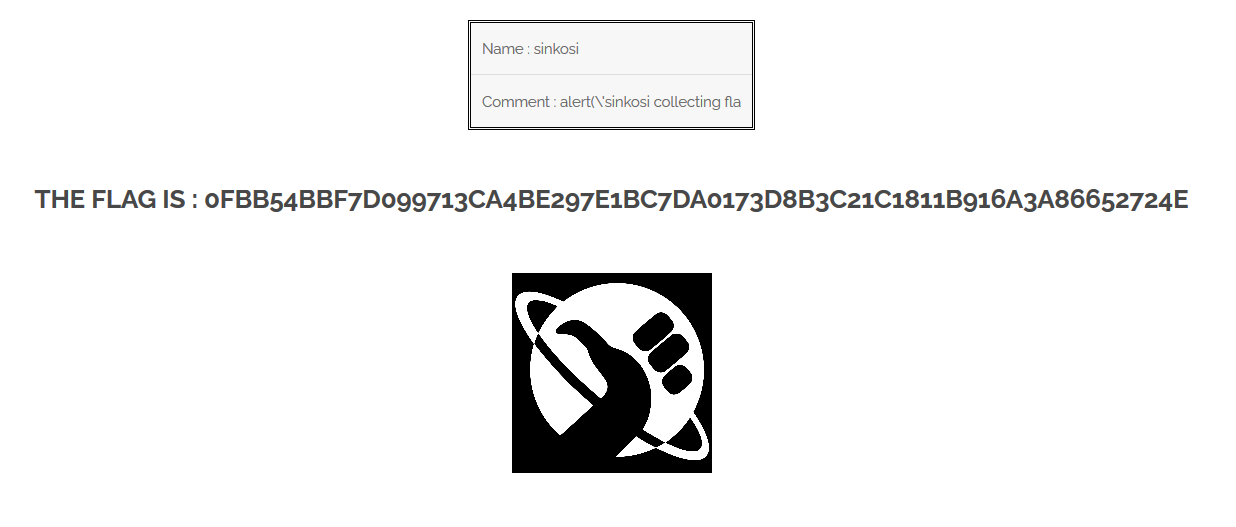
\includegraphics[width=0.5\textwidth]{06.Flag03/03-04.png}\\[0cm] 
\end{center}

\subsection{Vulnerability}

Cross-site scripting (XSS) is a type of security vulnerability typically found in web applications. XSS attacks enable attackers to inject client-side scripts into web pages viewed by other users. A cross-site scripting vulnerability may be used by attackers to bypass access controls such as the same-origin policy.

\subsection{Location}

http://<ip-address>:80/index.php?page=feedback

\subsection{Method}

In the feedback inputs, under name I input
'a' just to test. Under the Message slot I put in:

`<script>alert('sinkosi collecting flags');</script>`

This resulted in the flag popping out onto the screen.

\subsection{Tools}

\begin{figure}[!htb]
    \centering
    \subfloat[Landing]{
\includegraphics[width=.45\columnwidth]{06.Flag03/03-01.png}\label{fig: 03-01 - wtf}} \quad
    \subfloat[Feedback]{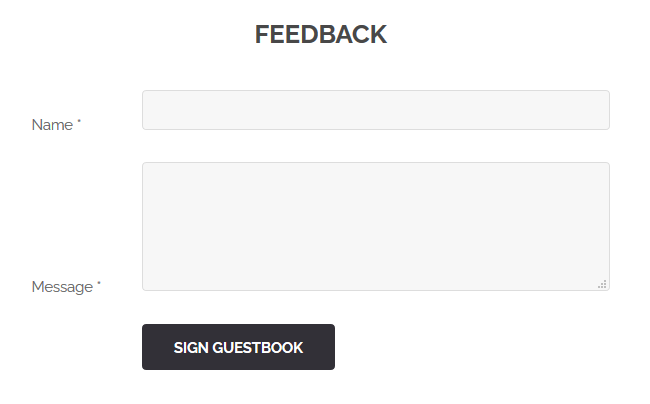
\includegraphics[width=.45\columnwidth]{06.Flag03/03-02.png}\label{fig: 03-02 - wrong}} \\
    \subfloat[Scripting...]{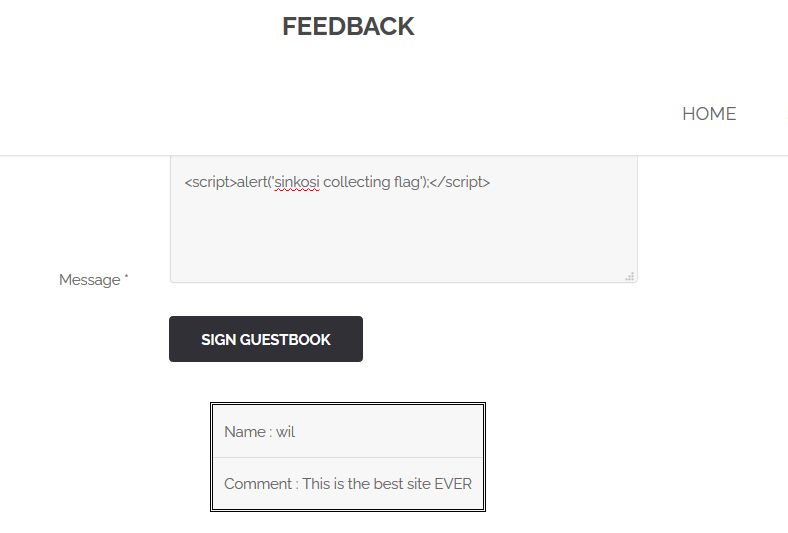
\includegraphics[width=.45\columnwidth]{06.Flag03/03-03.png}\label{fig: 03-03 - nope}} \quad
    \caption[Flag 03 Method]{Process to Capture the XSS Flag} % The text in the square bracket is the caption for the list of figures while the text in the curly brackets is the figure caption
    \label{fig:flag03 method}
\end{figure}


\begin{itemize}
    \item \href{https://en.wikipedia.org/wiki/Cross-site_scripting}{Wikipedia}
    \item \href{https://owasp.org/www-community/attacks/xss/}{OWASP}
    \item \href{https://portswigger.net/web-security/cross-site-scripting}{Portswigger}
\end{itemize}

\subsection{Remedy}

\begin{itemize}
    \item Filter input on arrival. At the point where user input is received, filter as strictly as possible based on what is expected or valid input.
    \item Encode data on output.
    \item Use appropriate response headers
    \item Content Security Policy
\end{itemize}

\paragraph{What can XSS be used for?}

An attacker who exploits a cross-site scripting vulnerability is typically able to:
\begin{itemize}
    \item Impersonate or masquerade as the victim user
    \item Carry out any action that the user is able to perform.
    \item Read any data that the user is able to access
    \item Capture the user's login credentials.
    \item Perform virtual defacement of the web site
    \item Inject trojan functionality into the web site.
\end{itemize}
